\chapter[Requirements]{Requirements analysis and specification}
\label{chap:requirements}
%ELSAM states that we should be sensitive to changes in the powergrid frequency, and be able to communicate using a network.
The ELSAM agreement states that the grid frequency must be 50Hz at all times . If the frequency is lower, our device should turn off unneeded loads or devices. ELSAM defines two types of loads; Normal operation reserve and Disturbance reserve.\\
The Normal operation reserve should be completely activated when the frequency drops 49.9Hz. Under these conditions it should turn off equipment, which is able to do so in 2-3 minutes or less. These devices would include equipment not crucial to production (e.g.heater or lighting ).\\ 
Disturbance reserve mode is used when the grid frequency does not return to normal state. In our case we turn off a battery powered device (a laptop) and try to make sure we dont empty their batteries completely before turning the power back on.

To make the ELSAM demands more accessible and more applicable to our assignment we have put the demands in to a hierarchy se Figure \ref{fig:reserver_demands} .\\ This makes it easy to see which requirements will be applied to the normal operation reserve and to the disturbance reserve. Many of the demands are not implemented yet, this means that the they should also be viewed as suggestion to further work.

\begin{figure}[!h]
  \centering
  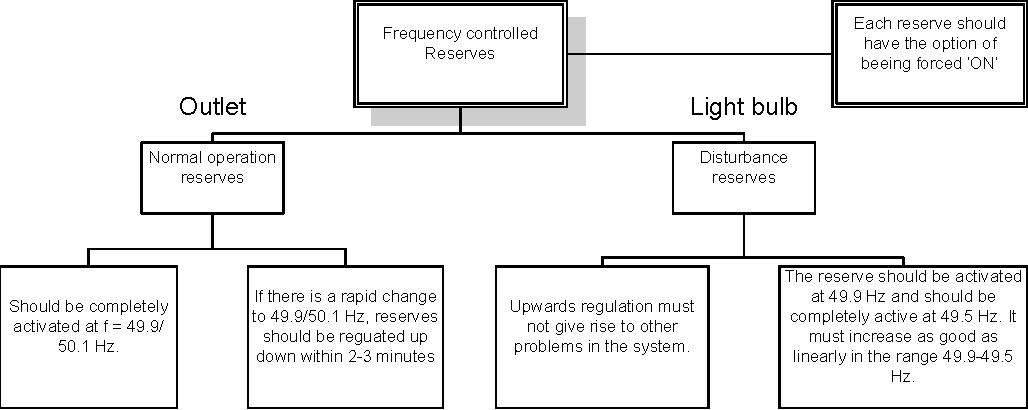
\includegraphics[width=0.9\textwidth]{figs/Demands_for_automatic_active_reserves.pdf}
  \caption{Hierarchy of the frequency controlled reserves in this report}
  \label{fig:reserver_demands}
\end{figure}
To be able to do more ``intelligent'' grid offloading, we must be able to communicate with the outside world. As there is no protocol specified, the logical choice would be tcp/ip for transport, as there is is already a well-established global infrastructure using this. The data should be transferred in an easy parsable format, such as XML.\\\\
Users of the device should also be able to view the status, current configuration and make changes to the configuration as well. The status and configuration should be available both from a physical interface and via a remote interface. As out device has a touchscreen it will serve the purpose as a physical interface, and the remote interface should be done in html.\\\\
This leaves us with the following requirements:
\begin{itemize}
\item Detect grid frequency, and respond to changes
\item Toggle relays based on frequency algorithm
\item Implement a TCP/IP stack
\item Implement a HTTP server
\item Design human interfaces for local access
\item Design human interfaces for remote access
\item Design machine interfaces for remote access
\end{itemize}

\section{Tools used}
An application development process' success or failure can depend largely on the tools used in the process. Good tools for documenting, debugging and versioning should be considered bare minimums.
\subsection{Debugging tools and methods}
When developing the communications interface we use the program ``wireshark'' \footnote{www.wireshark.org} to verify http requests and responses.\\
The board we will be using contains a JTAG port, for interactive debugging. This means we are able to stop the processor, read and modify registers or memory. This feature is extemly useful when debugging an application.

\subsection{Information scraping}
For doing quick notes on random information concerning code, documentation, requirements or specifications. We will be using a wiki for this purpose

\subsection{Versioning}
When developing an application, a versioning system is very useful both for experimenting with new features, because you have the ability to quickly roll-back to a working version. It is also a great way to do backup on your project.

%\section{Chapter Summary}  %% Should this be here ?
%\label{sec:SummaryChap2}



